\section{Overview of hardware}

The design for the final IoT system involved three distinct module types: Sensor
node, repeater and gateway. The system involves two separate sensor nodes that
are placed in range of the repeater. The repeater is then placed in range of an
internet-enabled gateway endpoint to allow the uploading of climate data to the
cloud.

\begin{figure}[H]
    \centering
    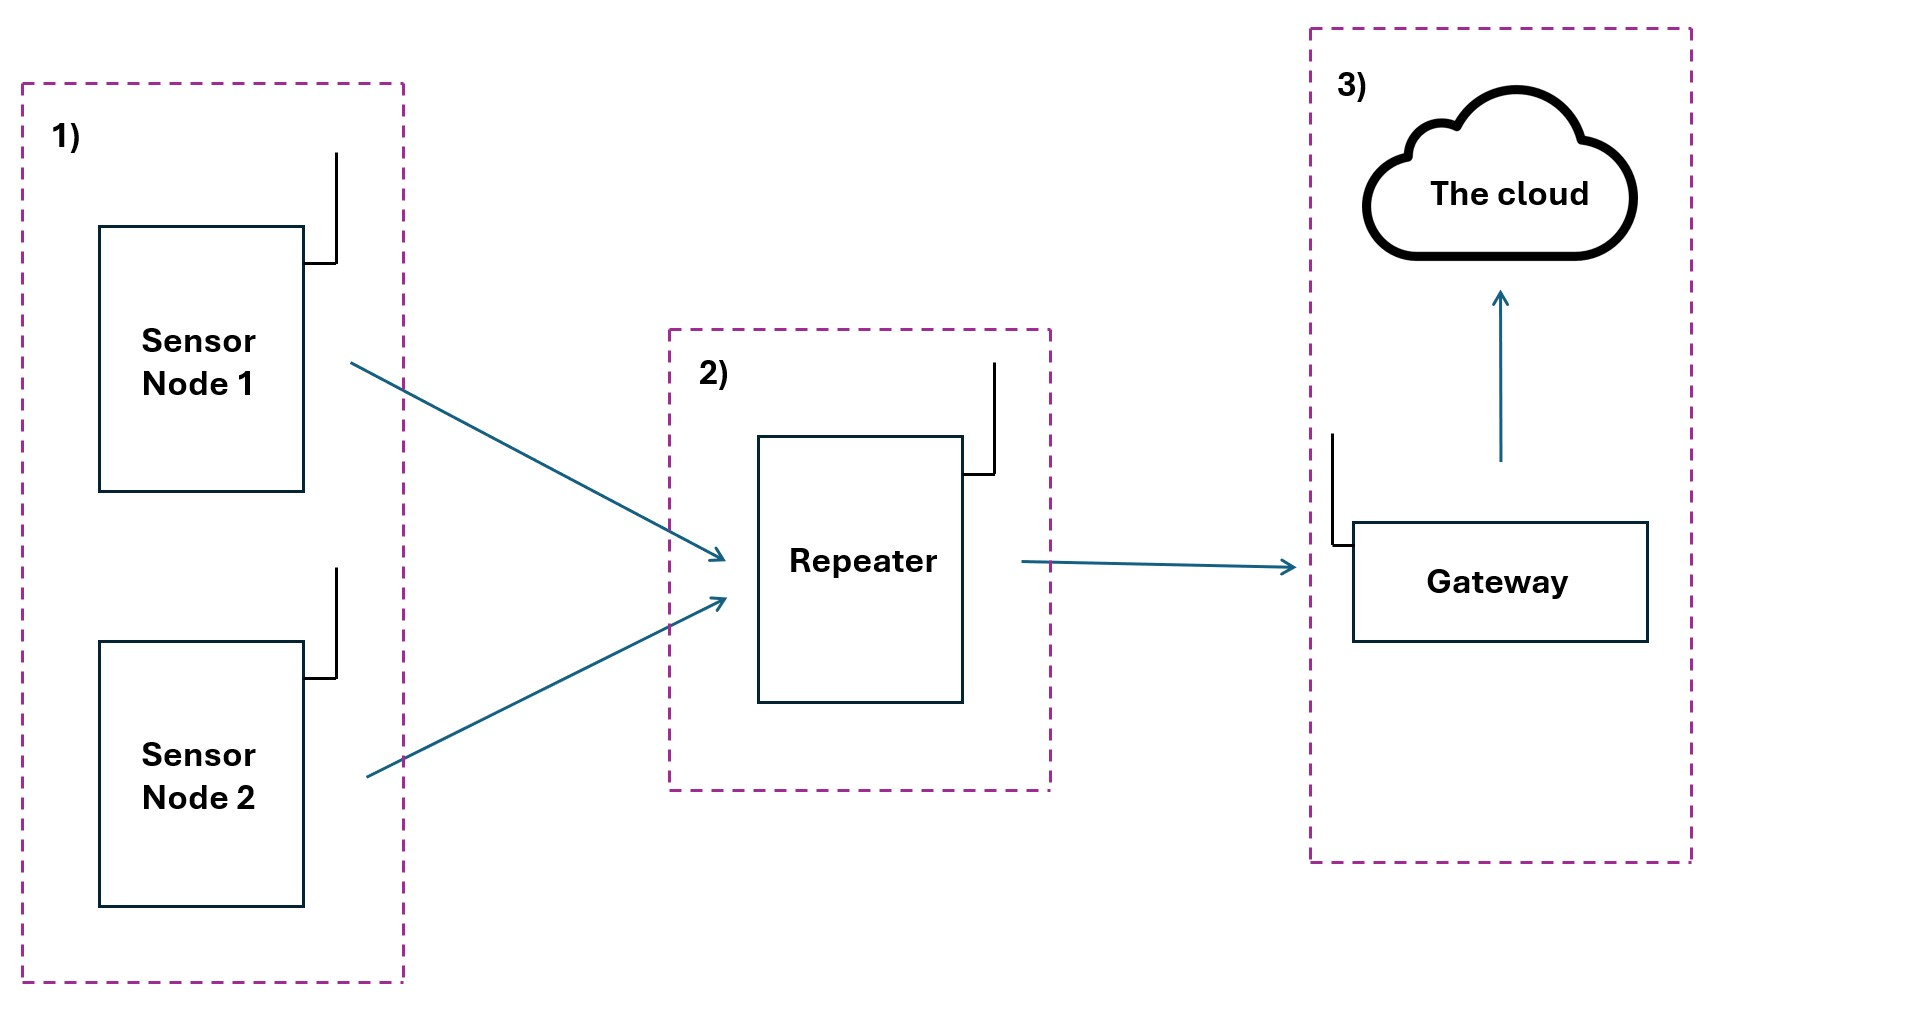
\includegraphics[width=0.9\textwidth]{contents/part-2/fig2/network-diagram.jpg}
    \caption{Network diagram of the system}
    \label{fig:network-diagram}
\end{figure}

\begin{enumerate}
    \item Sensor Node: The two nodes in this part of the network are in the
          perception layer. The nodes collect readings on temperature, humidity,
          wind speed and soil moisture levels. The results are collated into a
          comma separated string which is then emitted as a single packet from
          the LoRa transmitter.
    \item Repeater: This module is part of the network layer of the system as it
          facilitates communication between the perception layer and the
          application layer. The repeater is reads and decodes received LoRa
          signals from the sensor nodes. It then adds signal strength
          information to the string and re-emits the LoRa signal. The repeater
          has no sensors but is otherwise
    \item Gateway: The final part of the hardware system is the gateway - which
          is also part of the network layer. The gateway consists of a
          challenger to receive LoRa signals connected to a raspberry pi which
          can read the the decoded LoRa messages from the challenger's serial
          output. The raspberry pi also has a WiFi radio onboard so it is
          responsible for the uploading of data to the cloud.
\end{enumerate}



